\subsection{Investigating The Parameters of The SABR Model} \label{invest_sabr}
In this Section, we will explore the parameters of the SABR model. This analysis will offer insights into 
how different parameters influence the behavior of implied volatility. We will conduct this investigation using 
the closed-form solution established in the previous Section. Our study will be build on  \autoref{sigma_B} and 
\autoref{sigma_ff}, where we will test various parameter values. To see how changes in the different parameters
affects the implied volatility smile, we fix the values of the parameters during the study. 
The purpose of fixing the values of the parameters, is to isolate the change in the investigated parameter. 
Below in \autoref{tab:parameters} the chosen values of the parameters are listed, together with a short
explain of the parameters. Then the study is performed by changing the parameters one by one, to illustrate the 
isolated effect of the parameters. 
\\
\begin{table}[H]
    \centering
    \begin{tabular}{ccc}
      \toprule
      \textbf{Parameter} & \textbf{Parameter explanation} & \textbf{Value} \\
      \midrule
      \rowcolor{lightgray!40} $F$ & Initial forward rate or asset price & 100 \\
      $T$ & Time to maturity & 1 \\
      \rowcolor{lightgray!40} $K$ & Strike & $K \in (80,120)$ \\
      $\alpha_0$ & Initial level of volatility & 0.1 \\
      \rowcolor{lightgray!40} $\beta$ & Elasticity of the volatility & 0.5 \\
      $\rho$ & Correlation between the asset price and its volatility & -0.4 \\
      \rowcolor{lightgray!40} $\nu$ & Volatility of the volatility parameter & 0.25 \\
      \bottomrule
    \end{tabular}
    \caption{Summary of parameters used for investigating the SABR model}
    \label{tab:parameters}
\end{table}
\noindent
We will start the study with investigating how $\alpha_0$ affects the volatility smile in the SABR model. 
First we note that the fixed value of $\alpha_0$ is $0.1$ Hereafter we adjust the value of $\alpha_0$ to $0.08$ and $0.12$,
where the other parameters are kept fixed as listed in \autoref{tab:parameters} above. So having changed the parameter
up and down from the initial value of $\alpha_0$.
We note that the parameter $\alpha_0$
represents "the initial level of volatility" as it is the starting point for the stochastic volatility process. 
Below in \autoref{fig:alpha} the volatility smile is illustrated for three different value of $\alpha_0$. 
From \autoref{fig:alpha} we see that the up and down movements don't change the shape of the volatility smile, 
it only shifts the volatility smile respectively up and down given the movement in $\alpha_0$.
\begin{figure}[H]
    \centering
    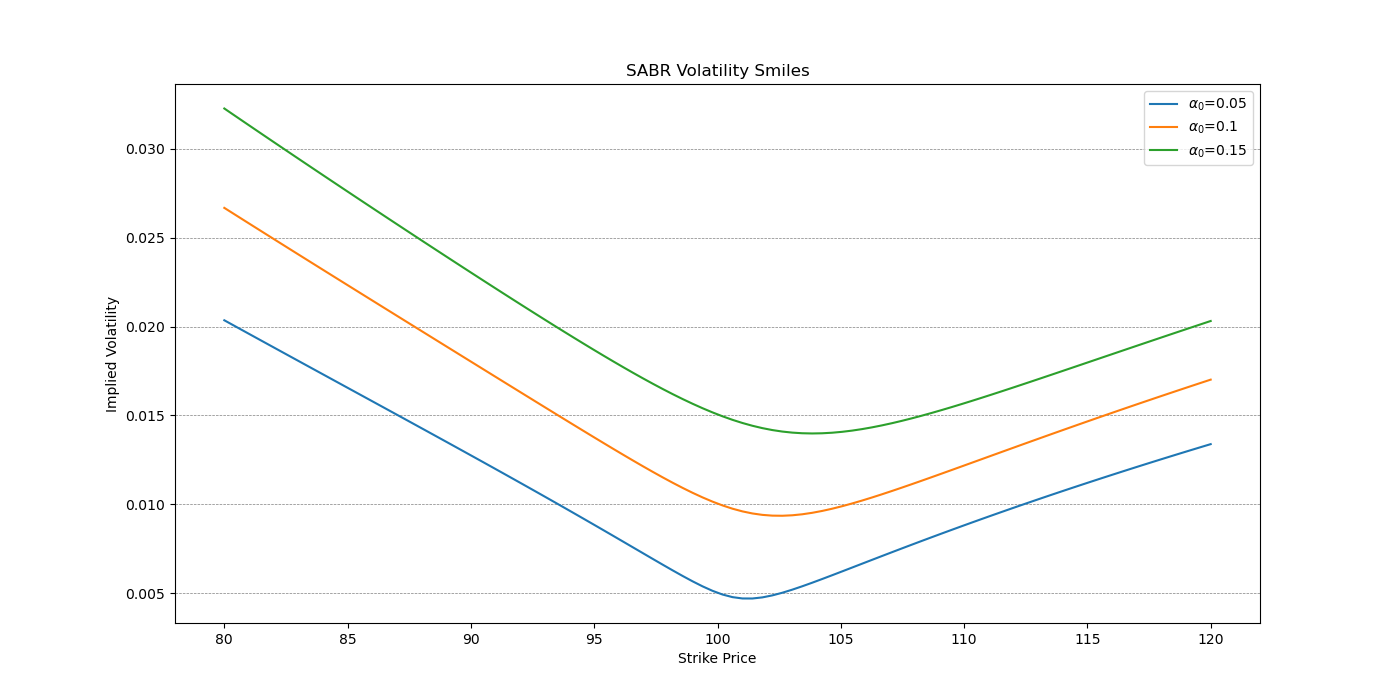
\includegraphics[scale =0.5]{/Users/nannaingemannohrt/Desktop/master_thesis/main/plots/SABR1_alpha.png}
    \caption{SABR model volatility smiles at various $\alpha_0$ levels}
    \label{fig:alpha}
\end{figure}
\noindent
Then we will continue the study of the parameters affects by looking into shift in the $\beta$ value in the SABR model.
Again we shift the value of $\beta$ up and down from the fixed $\beta$ in \autoref{tab:parameters}. So we will look at $\beta$ equal to $0.45$,
$0.5$ (the fix beta) and $0.55$. 
Although not explicitly constrained in the paper Managing Smile Risk 
of Hagen (2002) \cite{Smile} we restrict $\beta$ to the range $[0, 1]$. 
Choosing a $\beta$ less than 0 would lead to an illogical scenario where higher forward prices F result in a smaller 
relative change in the process $F_t$, thus we set the lower limit at $\beta \leq 0$. Similarly, a $\beta$ greater than 1 would 
suggest that the expected deviation from the current state of $F_t$ exceeds the product of volatility and the current 
forward level (times $\alpha_0 \sqrt{t}$), which is also impractical. Therefore, we set the upper limit at $\beta \geq 1$ \cite{Smile}.
\\\\
Below in \autoref{fig:beta} the volatility smile in the SABR model for the different beta values are illustrated.
From \autoref{fig:beta} we see a small effect of the curvature of the volatility smile. We also note that for higher 
beta the shift is larger, than for lower beta. We also note that the change in the beta parameter is more present in 
the left side from of strike value at-the-money (ATM). Other than that we see the same patterns from the change in 
the alpha parameter, namely the up and down shifts in the volatility smile, respectively to the movement in the 
beta parameter.
\begin{figure}[H]
    \centering
    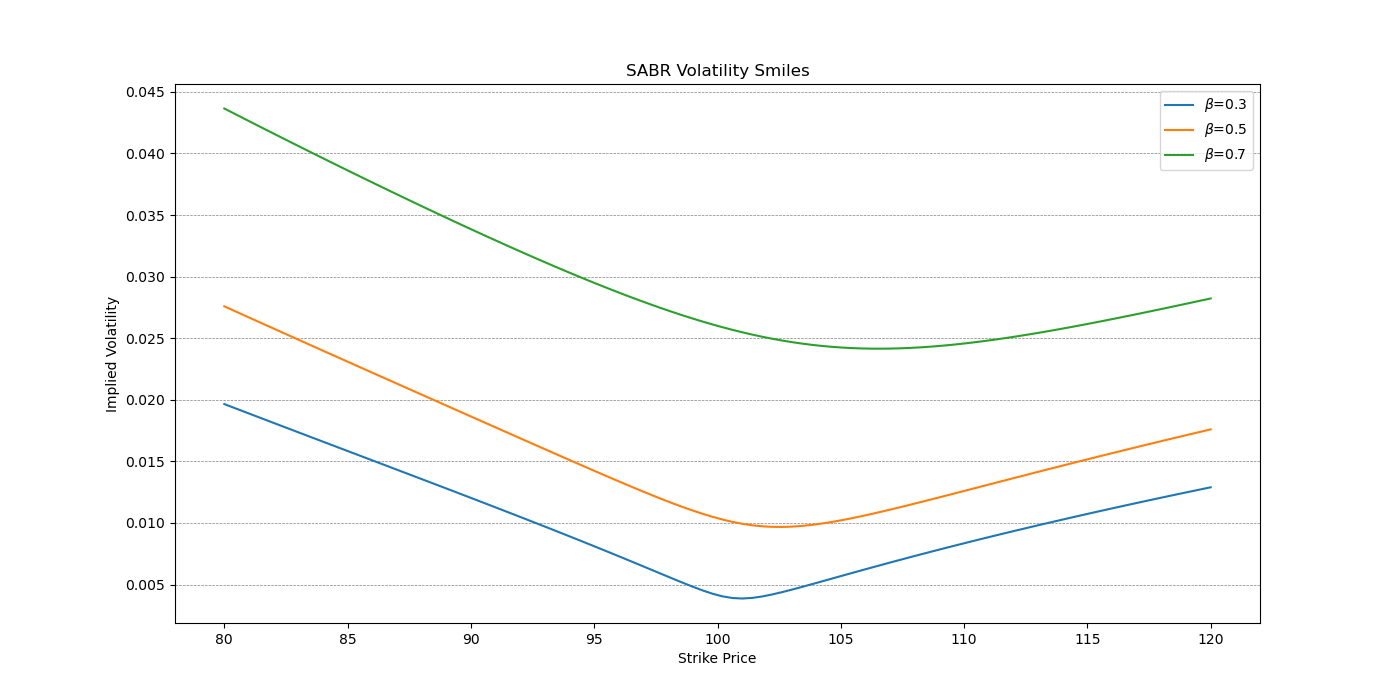
\includegraphics[scale =0.45]{/Users/nannaingemannohrt/Desktop/master_thesis/main/plots/SABR_beta.png}
    \caption{SABR model volatility smiles at various $\beta$ levels}
    \label{fig:beta}
\end{figure}
\noindent
Moving forward we will shift the $\nu$ parameter, which can be describe as the volatility of the volatility parameter.
Again we shift the $\nu$ parameter up and down from the fixed $\nu$ parameter listed in \autoref{tab:parameters}.
The volatility smile calculated from the SABR for the different $\nu$ parameters are illustrated in \autoref{fig:nu} below.
A very clear pattern emerges, namely that the parameter $\nu$ controls the curvature of the volatility smile in
the SABR model. When we looked at the shifts in the beta parameter we made a comment that it made small changes in 
the curvature. But after this part of the analysis, we clearly see that the curvature is determine from the value
of $\nu$. Which makes sense, when we think of the interpretation of the parameter describe before.
We also note that increasing $\nu$  increased the level of the implied volatility for the 
out-of-the-money (OTM) strikes also increase and vise vera.
\\\\
Then we look at the parameter for the correlation between the asset price and its volatility, namely $\rho$.
So we have that $\rho$ is the correlation between to two Wiener process in the SABR model, note
that $\rho$ is bounded and takes values between $-1$ and $1$. In \autoref{fig:rho} the shifted valus of $\rho$
from the fixed value is illustrated. 
We see that higher positive correlations generally show a decreasing trend in implied volatility with an increase in strike price, 
while strong negative correlations can cause the implied volatility to increase with strikes that are in-the-money (ITM).
We alo note that when the correlation is close to zero the smile is more symmetric around the ATM strike. 
So in total we see that the correlation parameter $\rho$ has a significantly affects on the shape and slope of
the volatility smile in the SABR model, and hence on the implied volatilities values.
\begin{figure}[H]
    \centering
    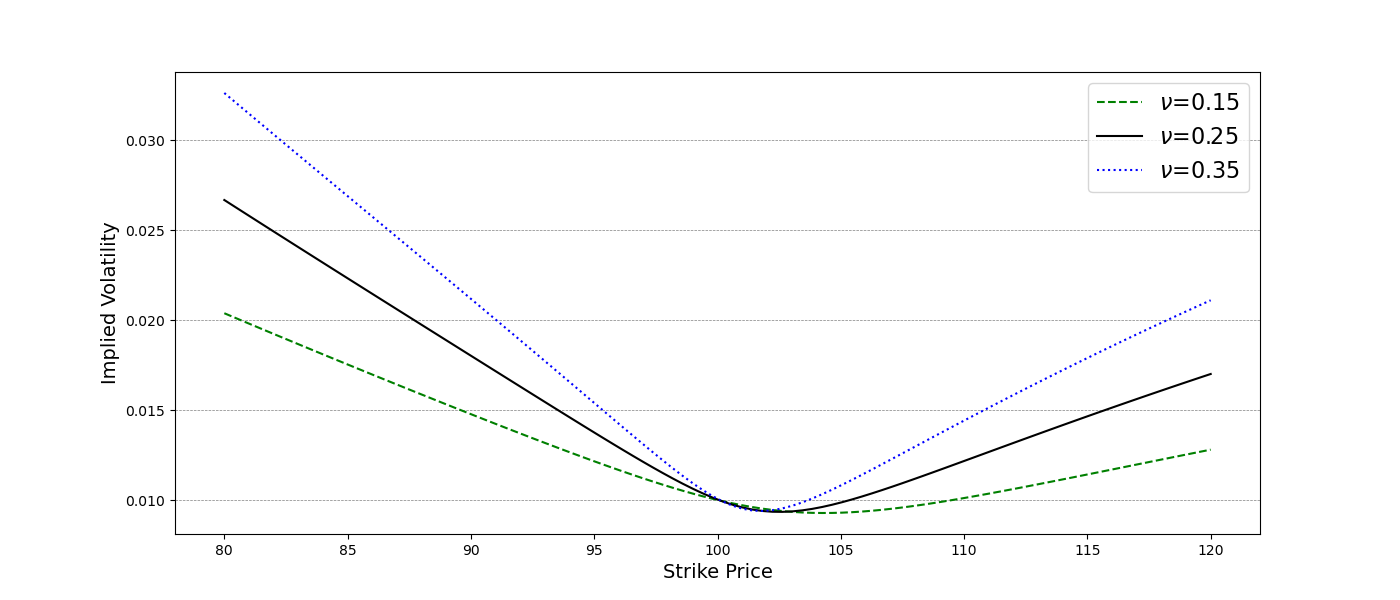
\includegraphics[scale =0.45]{/Users/nannaingemannohrt/Desktop/master_thesis/main/plots/SABR_nu.png}
    \caption{SABR model volatility smiles at various $\nu$ levels}
    \label{fig:nu}
\end{figure}

\begin{figure}[H]
    \centering
    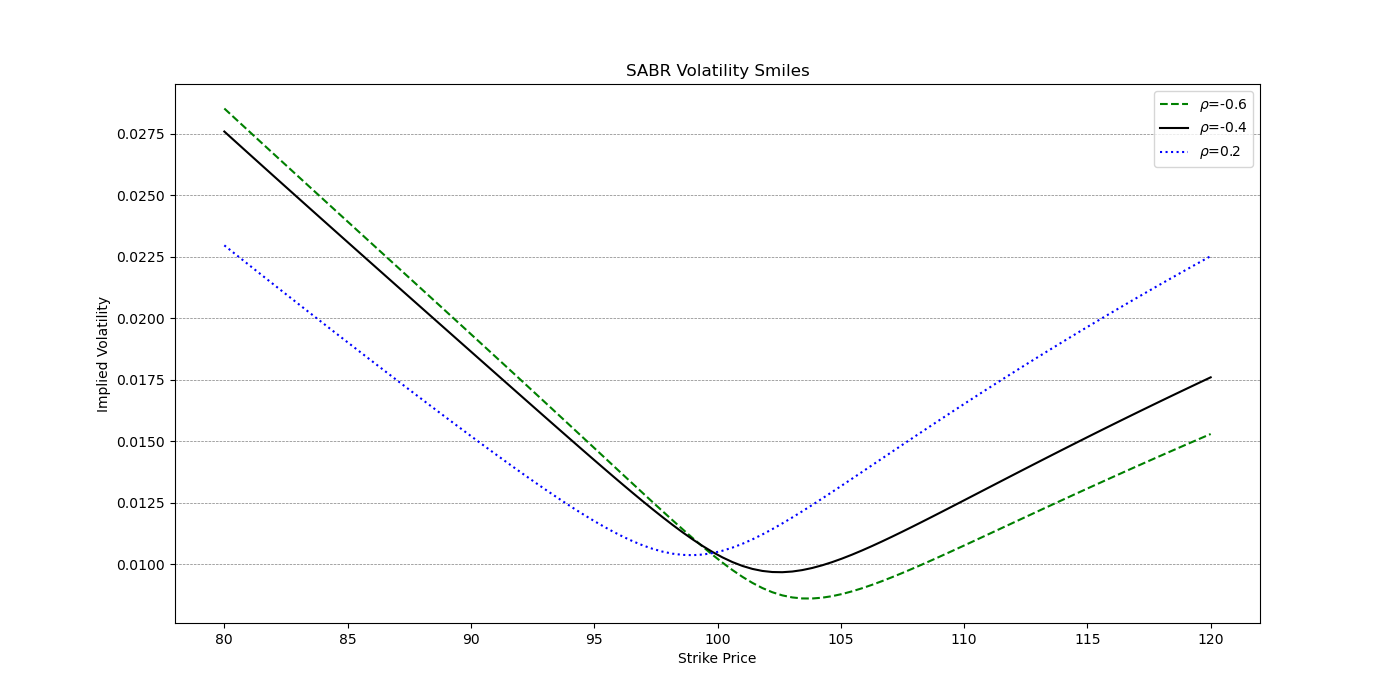
\includegraphics[scale =0.45]{/Users/nannaingemannohrt/Desktop/master_thesis/main/plots/SABR_rho.png}
    \caption{SABR model volatility smiles at various $\rho$ levels}
    \label{fig:rho}
\end{figure}

\begin{figure}[H]
    \centering
    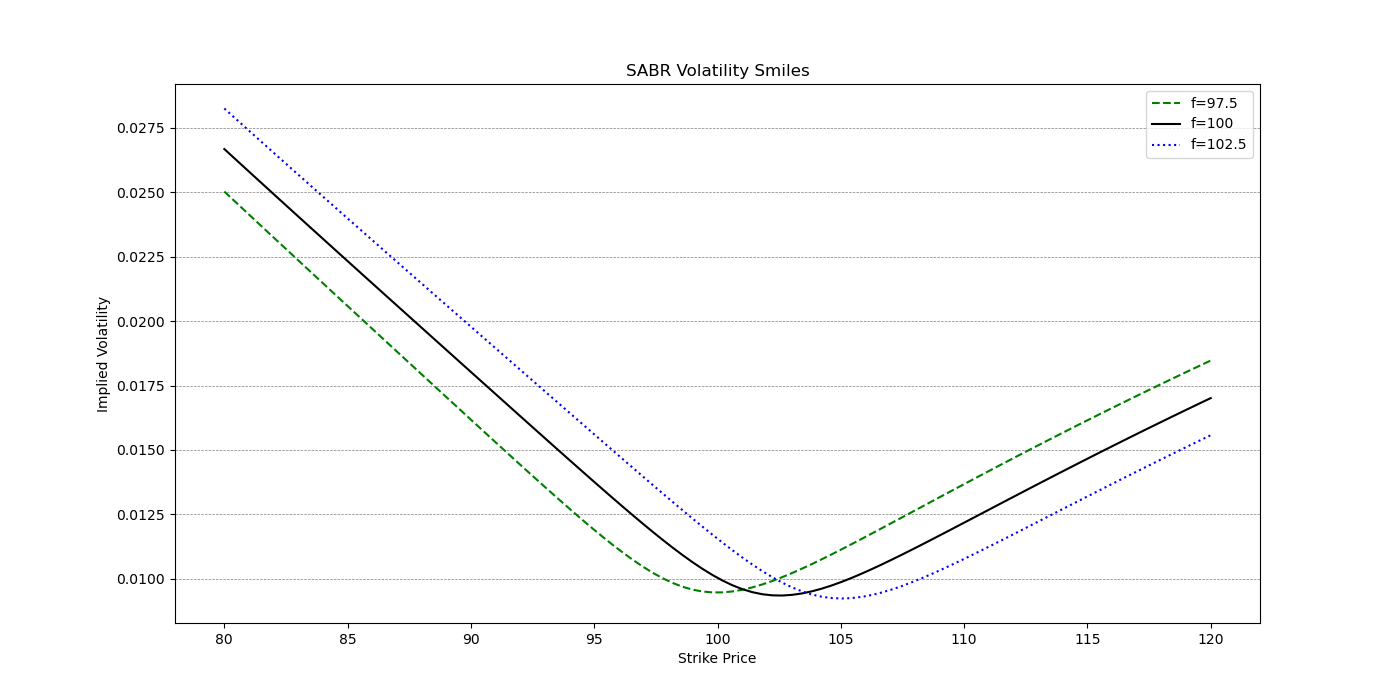
\includegraphics[scale =0.45]{/Users/nannaingemannohrt/Desktop/master_thesis/main/plots/SABR_f.png}
    \caption{SABR model volatility smiles at various F levels}
    \label{fig:f}
\end{figure}
\noindent
Finally we will investigate how the forward price, F, affect the volatility smile in the SABR model. 
The same procedure as for the other parameters will be used. So in \autoref{fig:f} the volatility smile
for the forward prices are illustrated. We see that the slope, shape and curvature is retained, when there
is only change in the forward price. Which is as we expected given how the forward price, F, enters in the closed
solution for the implied volatility in \autoref{sigma_B} and \autoref{sigma_ff}.
\\\\
To summarize this Section provides knowledge of the impact of the various parameters in the closed-form solution
for the implied volatility in the SABR model. This knowledge gives a good idea of how the model works, and 
positions us better to understand estimations of the model. So now we have looked at the closed-form solution and 
are ready for the next step of our analysis which is to look at  estimating the parameters in the SABR model.
\newpage
\subsection{Estimating Parameters in The SABR Model} \label{est_parm_sabr}
In this Section we will look into how we can estimate the parameters in the SABR model.
So we want to estimate $\alpha$, $\beta$, $\rho$ and $\nu$.       
There are different methods for estimating the parameters in the SABR model. 
The various approaches distinguish themselves based on their methods for estimating or selecting $\beta$ and $\alpha$.
$\beta$ may be either set to a predetermined best guess or fitted together with other parameters.
Similarly, $\alpha$ may be estimated using \autoref{sigma_atm} or fitted concurrently with the other parameters.
\\\\
We will apply the approach, where we chose some fixed $\beta$'s and the estimate $\alpha$ using \autoref{sigma_atm}  and the
setup a minimization problem there minimize $\rho$ and $\nu$. We chose this approach since earlier in Chapter \ref{invest_sabr}
we noticed that changes in $\beta$ and $\rho$ gave some of the same effect on the volatility smile. Therefor we chose to fixe  $\beta$, for different
values of $\beta$. Let's then remind yourself of what the change in $\beta$ did to the volatility smile.
We saw that when moving the $\beta$ value op and down, the corresponding change in the volatility smile appeared. 
Then we remind yourself of the dynamic of the forward rate in the SABR model, listed in \autoref{f_dyn}. 
Where we consider the term  $\alpha_t F_t^\beta$ as the total volatility of the forward rate process,
it becomes apparent that decreasing $\beta$ generally amplifies the volatility and vise vera. 
\\\\
Then we consider the minimization problem to estimate the SABR model, where the objective is to align
the market implied volatilities with the SABR model's volatility, which is computed for a 
set of strikes and the current forwards rate for combination of expiry and tenor \cite{Lindstrom}. 
Below the minimization problem is present with the parameters condition we argued for in Chapter \ref{invest_sabr}.
 
\begin{align}
   \min_{\rho, \nu} \sum_{i=0}^{N_k} \Big(\sigma_{\text{B}} - 
    \sigma_{\text{SABR}}(f, \sigma_{\text{ATM}}, k_i, T, \rho, \nu)\Big)^2 \\
    0 \leq \beta \leq 1, \quad -1 \leq \rho \leq 1, \quad 0 \leq \nu, \quad 0 \leq \alpha
\end{align}
There are also different approaches to estimating the $\alpha$ parameter.
To estimate $\alpha$ we will use the method proposed in the paper Managing Smile Risk 
of Hagen (2002) \cite{Smile},
where the ATM SABR-formula is inverted numerically. The ATM SABR-formula is listed in \autoref{sigma_atm} \cite{Smile}.
This is performed in \autoref{sigma_atm} to \autoref{ABC} below.
Another way to estimate $\alpha$ is to solve the 
minimization problem, but this will not be covered in the thesis.

\begin{align}
    \sigma_{\text{ATM}}  & = \frac{\alpha}{f^{1-\beta}} \left\{ 1 +
     \left[ \frac{(1-\beta)^2 \alpha^2}{24 f^{2-2\beta}} + \frac{\rho \beta \nu \alpha}{4 f^{1-\beta}}
      + \frac{(2-3\rho^2) \nu^2}{24} \right] t_{\text{ex}} \right\} \label{sigma_atm} \\
      0 &= A \cdot \alpha^3 + B \cdot \alpha^2 + C \cdot \alpha - \sigma_{\text{ATM}} f^{1-\beta}
\end{align}
where

\begin{align}
    A = \frac{(1-\beta)^2 T}{24 f^{2-2\beta}},
    \quad B = \frac{\rho \beta \nu T}{4 f^{1-\beta}},
    \quad C = \left[ 1 + \frac{2-3\rho^2}{24} \nu^2 \right] t_{\text{ex}} \label{ABC}
\end{align}
Before we are ready to estimate the parameters numerically, let's first take a short look at the required 
data to performed the estimation study. As mentioned we need the current forward rates for any combination 
of expiry and tenor. In this analysis we will consider data where the expiry is ten years and has various tenors 
namely [1Y,2Y,3Y,5Y,7Y,10Y,12Y,15Y,20Y,30Y]. Below in \autoref{tab:farward_parm} the describe forward rates is 
present. To illustrated the development of the forward rates over the different tenors, these are illustrated
in \autoref{fig:forward_plot} below. From the plot we see that the level of the forward rate is higher for
shorter tenors than longer durations tenors.
\\
\begin{table}[H]
    \centering
    \scalebox{0.85}{
    \begin{tabular}{ccccccccccc}
      \toprule
      \textbf{ Tenor} & 1Y & 2Y & 3Y & 5Y & 7Y & 10Y & 12Y & 15Y & 20Y & 30Y \\
      \midrule
      \textbf{ Forward rate}&0.2938 & 0.2976 & 0.2996 &0.2992 &0.2943 &0.2840 
      &0.2763 & 0.2654& 0.2517 & 0.2340\\
      \bottomrule
    \end{tabular}
    }
    \caption{Forward rates for ten years to expiry and various tenors. Data source Citi Velocity 21.02.2024}
    \label{tab:farward_parm}
\end{table}
\begin{figure}[H]
    \centering
    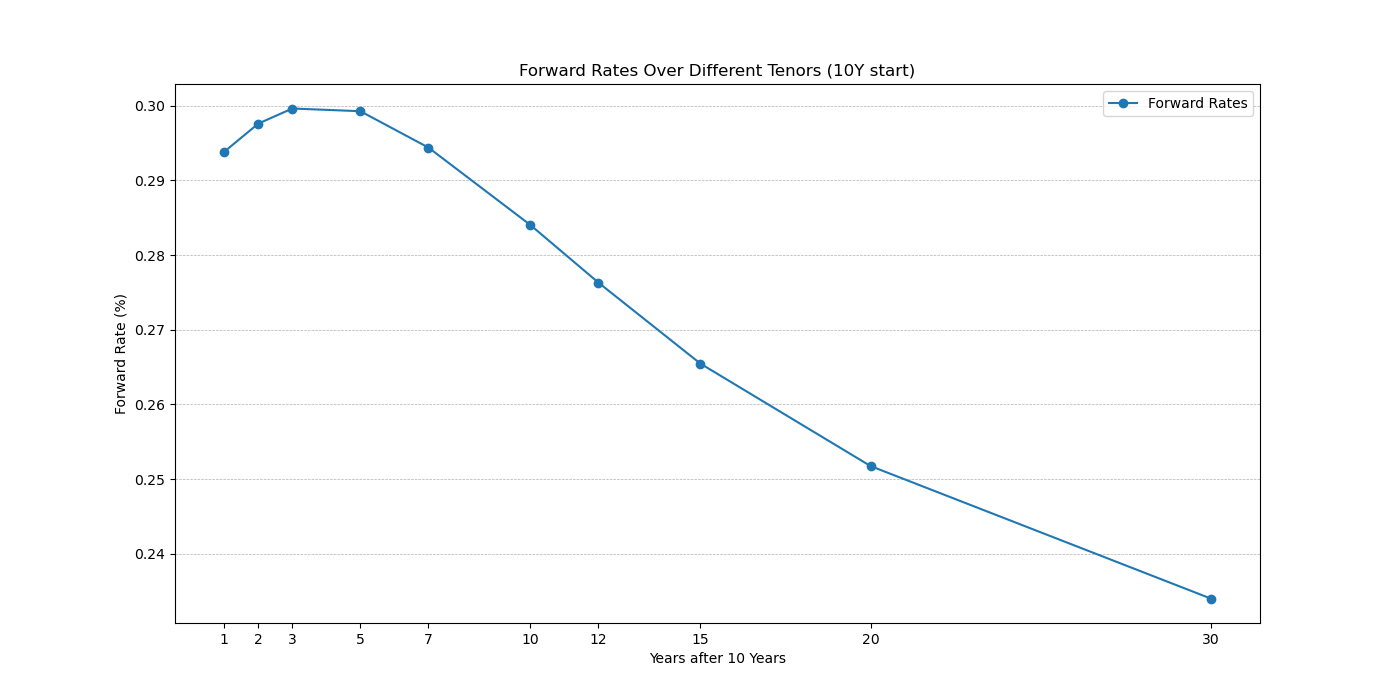
\includegraphics[scale =0.45]{/Users/nannaingemannohrt/Desktop/master_thesis/main/plots/forward_rates.png}
    \caption{Forward rates for ten years to expiry and various tenors. Data source Citi Velocity 21.02.2024}
    \label{fig:forward_plot}
\end{figure}
\noindent
So we have chosen the method where we chose a fixed $\beta$, so we chose the fixed $\beta$'s to be 0.5 and 1.
And then we performed the described estimation for the parameters $\alpha$, $\rho$ and $\nu$. 
This estimation was performed across various combinations of expiry and tenors, 
resulting in two separate tables that display the estimated parameters when $\beta$ is fixed at either 0.5 or 1. 
The estimated values for $\alpha$, $\rho$, and $\nu$, with $\beta$ fixed at 0.5, are presented in \autoref{tab:beta_0.5}. 
Similarly, the values for when $\beta$ is fixed at 1 are shown in \autoref{tab:beta_1}.
\\\\
Lets first comment on the estimated values in  \autoref{tab:beta_0.5}, where $\beta=0.5$.
The estimated parameters show generally moderate values for $\alpha$ across different tenor-expiry combinations, 
with a slight tendency to increase for longer expiries. The $\rho$ estimated values are predominantly positive, 
suggesting that higher rates correlate with higher volatility. Finally $\nu$  estimated values are high, 
indicating substantial volatility skew, which might suggest expectations of greater changes in 
rate movements over these periods. Then lets comment on the estimated values in \autoref{tab:beta_1}, where $\beta=1$.
In this case, the estimated $\alpha$ values are relatively higher compared to $\beta$ = 0.5, suggesting increased erratic behavior in volatility 
for these scenarios. The $\rho$ estimated  values are also positive but exhibit a wider range across different tenors and expiries. 
The estimated $\nu$ values remain high, reinforcing the presence of a significant volatility skew.
\\
\begin{table}[H]
    \centering
    \begin{tabular}{cccc}
      \toprule
      \textbf{Expiry x Tenor } & \textbf{$\hat{\alpha}$} & \textbf{$\hat{\rho}$}  & \textbf{$\hat{\nu}$} \\
      \midrule
      \rowcolor{lightgray!40}  10Y x 1Y &0.2526 & 0.3711 & 3.8123 \\
      10Y x 2Y &0.2516 & 0.3546 & 3.7993 \\
      \rowcolor{lightgray!40}  10Y x 3Y  &0.2460 & 0.3367 & 3.7752 \\
      10Y x 5Y &0.2394 & 0.3030 & 3.7173 \\
      \rowcolor{lightgray!40} 10Y x 7Y &0.2278 & 0.2762 & 3.7246 \\
      10Y x 10Y &0.2130& 0.2368 & 3.73220 \\
      \rowcolor{lightgray!40}  10Y x 12Y &0.2129 & 0.2461& 3.445 \\
      10Y x 15Y &0.2007 & 0.2201 & 3.6347 \\
      \rowcolor{lightgray!40} 10Y x 20Y &0.1939 & 0.2048 & 3.5607 \\
      10Y x 30Y &0.1881 & 0.1942 & 3.4496 \\
      \bottomrule
    \end{tabular}
    \caption{$\hat{\alpha}$, $\hat{\rho}$ and $\hat{\nu}$ for fixed $\beta$ = 0.5, using the SABR model.}
    \label{tab:beta_0.5}
\end{table}
\noindent

\begin{table}[H]
    \centering
    \begin{tabular}{cccc}
      \toprule
      \textbf{Expiry x Tenor} & \textbf{$\hat{\alpha}$} & \textbf{$\hat{\rho}$}  & \textbf{$\hat{\nu}$}\\
      \midrule
      \rowcolor{lightgray!40} 10Y x 1Y &0.4577 & 0.3114 & 3.6282 \\
      10Y x 2Y  &0.4535 & 0.2947 & 3.6284 \\
      \rowcolor{lightgray!40} 10Y x 3Y  &0.4426 & 0.2772 & 3.6199\\
      10Y x 5Y  &0.4320 & 0.2429 & 3.5869 \\
      \rowcolor{lightgray!40} 10Y x 7Y  &0.4153 & 0.2176 & 3.6137 \\
      10Y x 10Y &0.3962& 0.1799 & 3.6463 \\
      \rowcolor{lightgray!40} 10Y x 12Y &0.4420 & 0.1762 & 3.3525\\
      10Y x 15Y & 0.3865 & 0.1623 & 3.3560 \\
      \rowcolor{lightgray!40} 10Y x 20Y &0.3838 & 0.1456 & 3.4955 \\
      10Y x 30Y &0.3867 & 0.1221 & 3.3960 \\
      \bottomrule
    \end{tabular}
    \caption{$\hat{\alpha}$, $\hat{\rho}$ and $\hat{\nu}$ for fixed $\beta$ = 1, using the SABR model.}
    \label{tab:beta_1}
\end{table}
\noindent
\newpage
\noindent
The analysis of the SABR model parameters, specifically at fixed $\beta$ values of 0.5 and 1, 
reveals distinctive volatility dynamics and correlation structures across various tenor-expiry combinations. 
At both $\beta$ values, the presence of a positive $\rho$ indicates that rate increases are likely correlated with heightened volatility.
The notable distinctions at $\beta$ = 1 are the higher $\alpha$ and $\nu$ values, suggesting a more erratic behavior and pronounced 
skewness in volatility. These characteristics are particularly significant for pricing and risk management in scenarios 
anticipating substantial rate dynamics. The insights garnered from this analysis are crucial for financial institutions and 
investors involved in hedging, pricing, or trading derivatives influenced by these model dynamics.
\\\\
To end this section we will look at estimated parameters despited by the volatility smile. 
We chose to look a the volatility smile, for estimated values where $\beta$ was fixed to be 0.5. 
Since this is the most common choice for $\beta$. We despited the combination where the tenor is 10 years, in large format in 
\autoref{fig:10y_plot_smile} below and all combined of the swaption volatility smile with expiry in 10 years, and the 
various tenors are despited in \autoref{fig:10Y1Y_} to \autoref{fig:10Y10Y_} below. 
From \autoref{fig:10y_plot_smile}  we see that estimated volatility smile fits the market data good, which make sense from 
how we estimated the parameters to find the volatility smile. We note that estimated values for $\nu$ in both 
\autoref{tab:beta_0.5} and \autoref{tab:beta_1}, are relative high. But this align with the steepness or level we see the in the 
volatility smile in the market data. The volatility smile tends to be more convex when $\nu$ is large and this is clearly 
the case here. This tendency appearers in  most of the volatility smile despited in \autoref{fig:10Y1Y_} to \autoref{fig:10Y10Y_}.
But again we also see for the tenor-expiry combination for longer tenor, has not the same steepness in the level in 
the volatility smile. For the longer durations tenor combination we see a more symmetric volatility smile around the
ATM strike. We also note the the changes in the volatility smile i larger for the OTM strike, than for the ITM strikes. 
\\\\
Then we should ask yourself how does the  steepness or level we see the in the 
volatility smile in the market data affects the price of a swaption. When we are determine swaption we should also consider 
with sensitivities there are related to the price of the swaption. The above analysis pointing at there could 
be a sensitive related to $\nu$. Therefor the next step in the analysis is to look closer at the models sensitivities. 
But first a look at how swaption prices change over various tenors in Chapter \ref{swaption_price_sec}.

\begin{figure}[H]
    \centering
    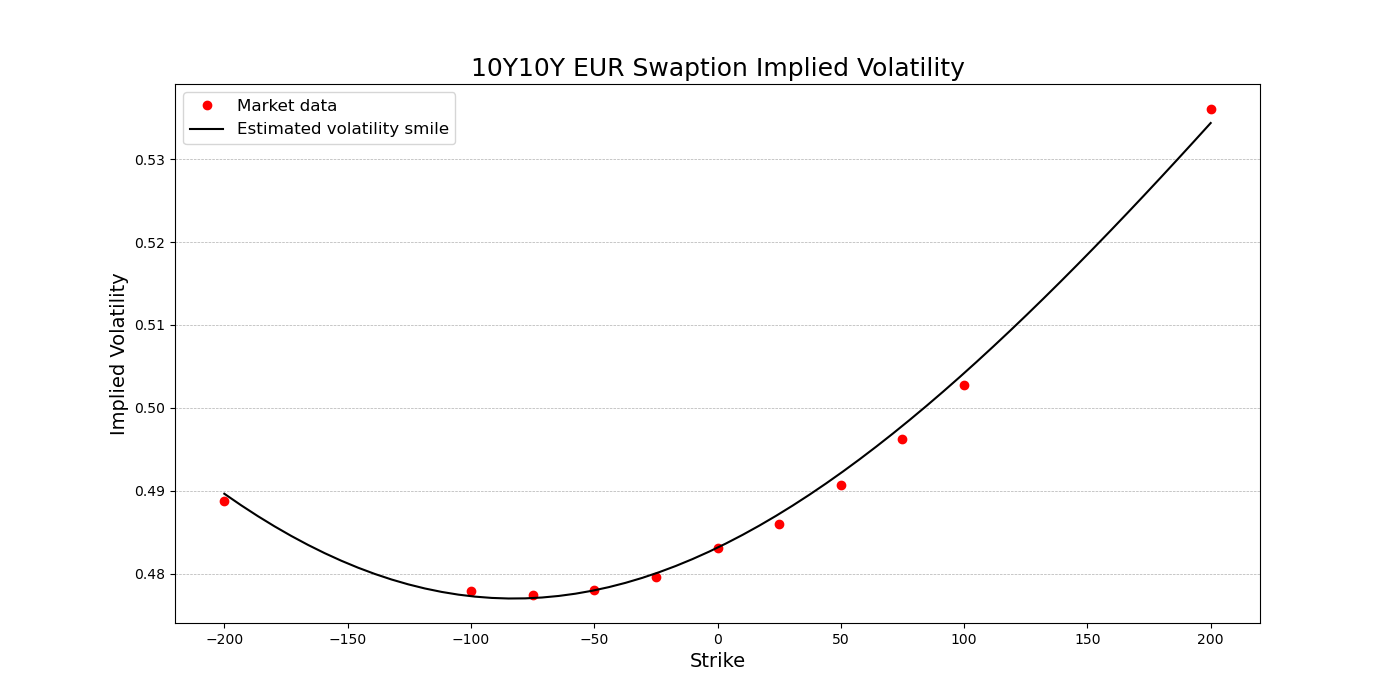
\includegraphics[scale = 0.5]{/Users/nannaingemannohrt/Desktop/master_thesis/main/plots/10Y10Y_est.png}
    \caption{Estimated implied volatility smile for a 10Y10Y EUR swaption using the SABR model. \\Beta fixed at 0.5.
    Data source Citi Velocity 21.02.2024}
    \label{fig:10y_plot_smile}
\end{figure}
\noindent


\begin{figure}[htbp]
    \centering
    \begin{subfigure}{0.43\textwidth}
        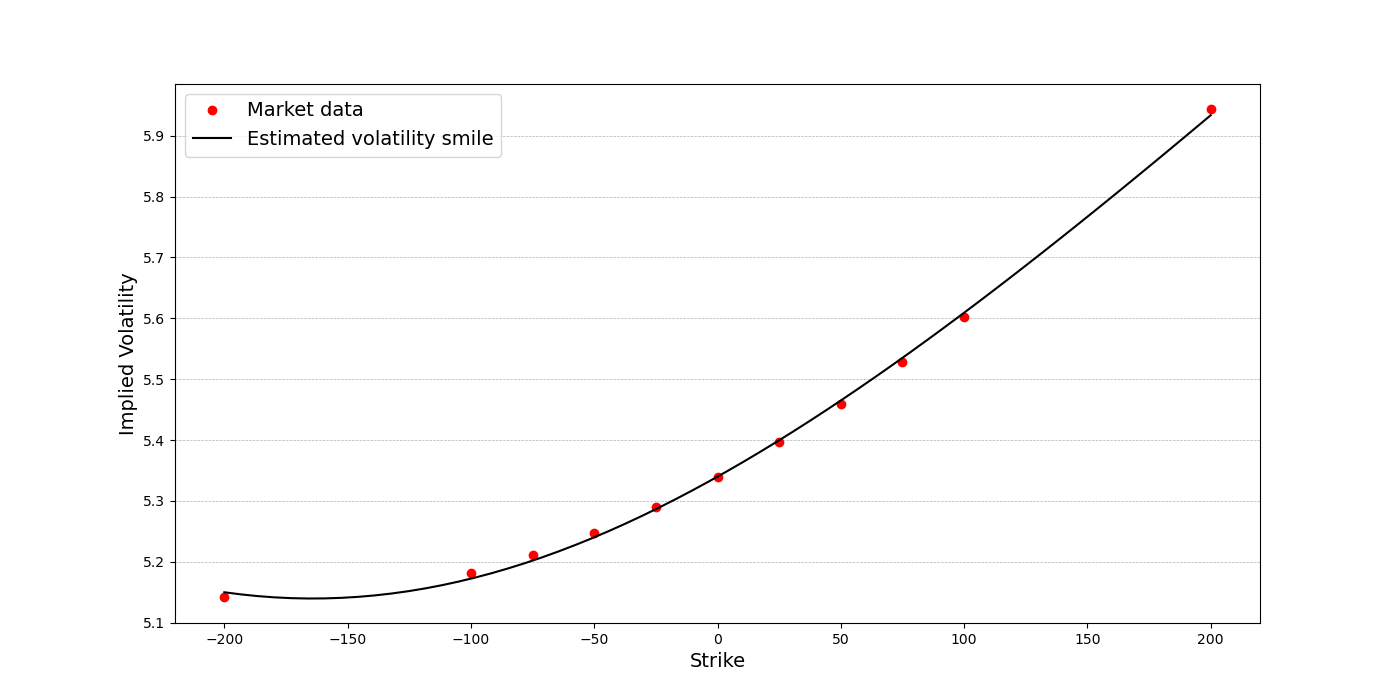
\includegraphics[scale =0.22]{/Users/nannaingemannohrt/Desktop/master_thesis/main/plots/10Y1Y_est.png}
        \caption{Volatility Surface EUR swaption 10Y1Y}
        \label{fig:10Y1Y_}
    \end{subfigure}\hfill
    \begin{subfigure}{0.43
        \textwidth}
        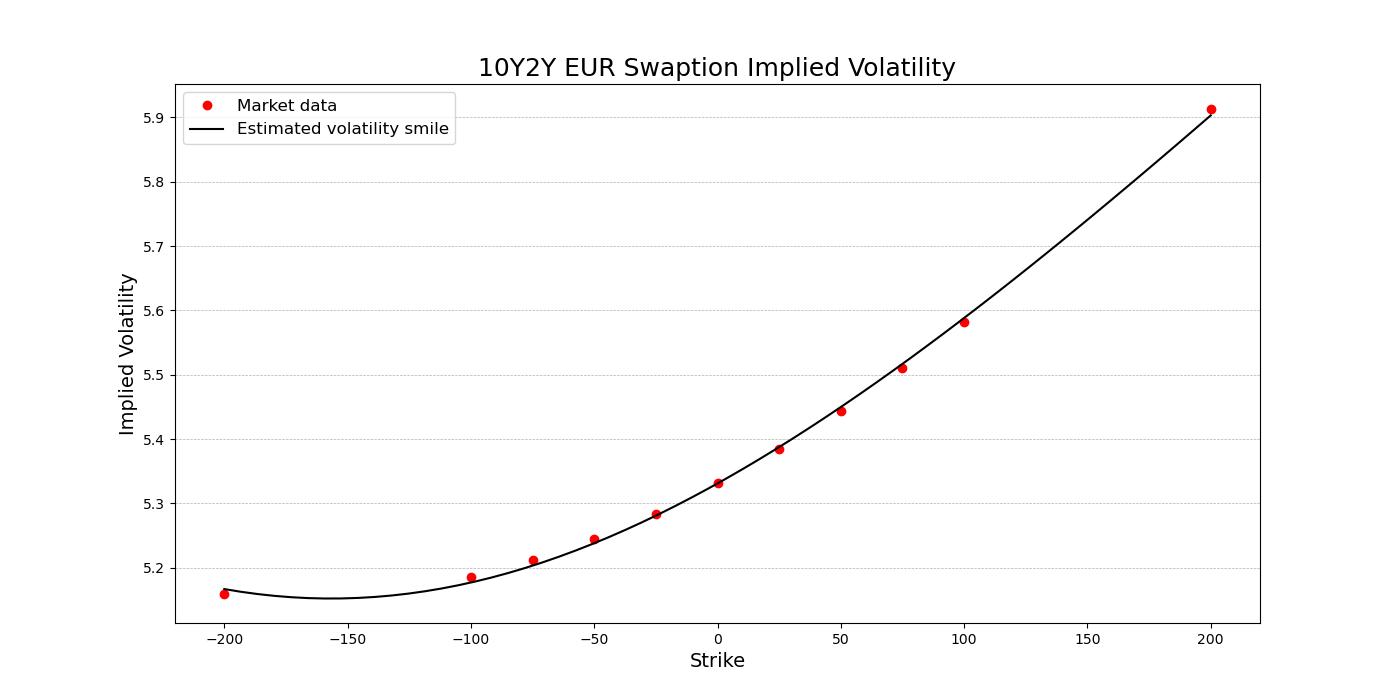
\includegraphics[scale =0.22]{/Users/nannaingemannohrt/Desktop/master_thesis/main/plots/10Y2Y_est.png}
        \caption{Volatility Surface EUR swaption 10Y2Y}
        \label{fig:10Y2Y_}
    \end{subfigure}
    \begin{subfigure}{0.43\textwidth}
        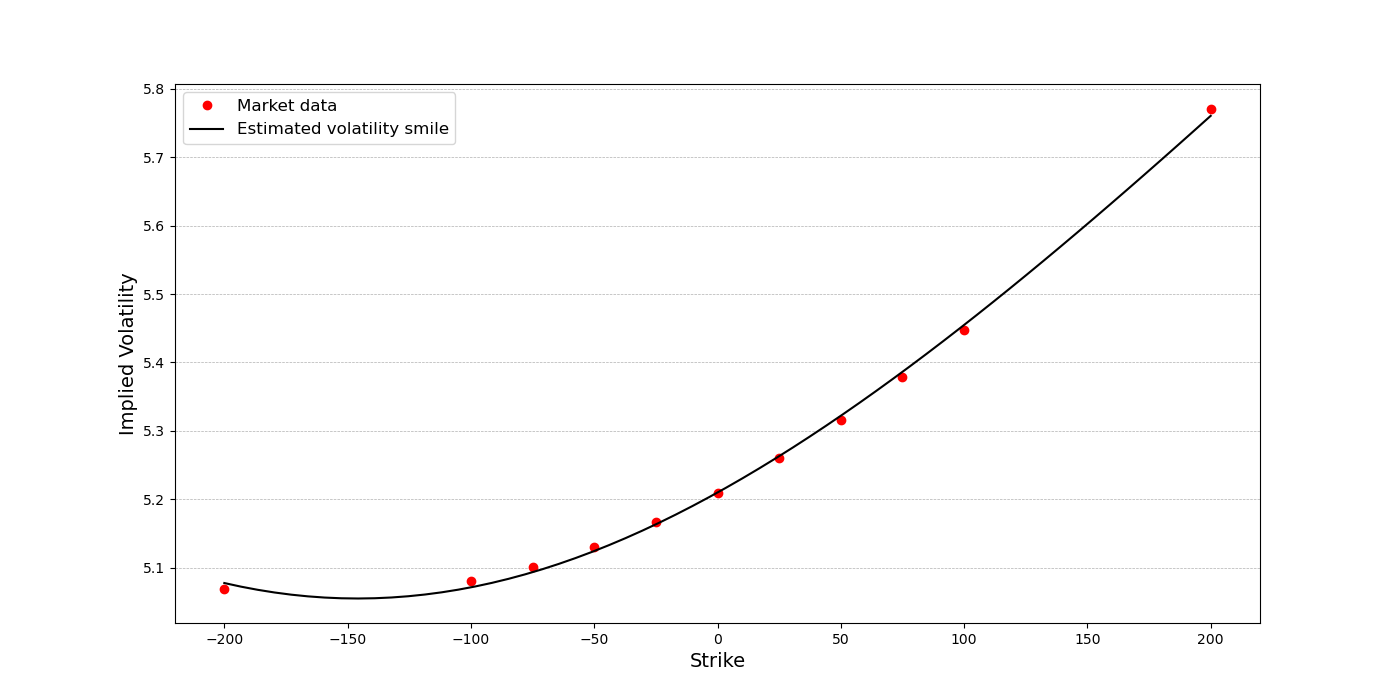
\includegraphics[scale =0.22]{/Users/nannaingemannohrt/Desktop/master_thesis/main/plots/10Y3Y_est.png}
        \caption{Volatility Surface EUR swaption 10Y3Y}
        \label{fig:10Y3Y_}
    \end{subfigure}\hfill
    \begin{subfigure}{0.43\textwidth}
        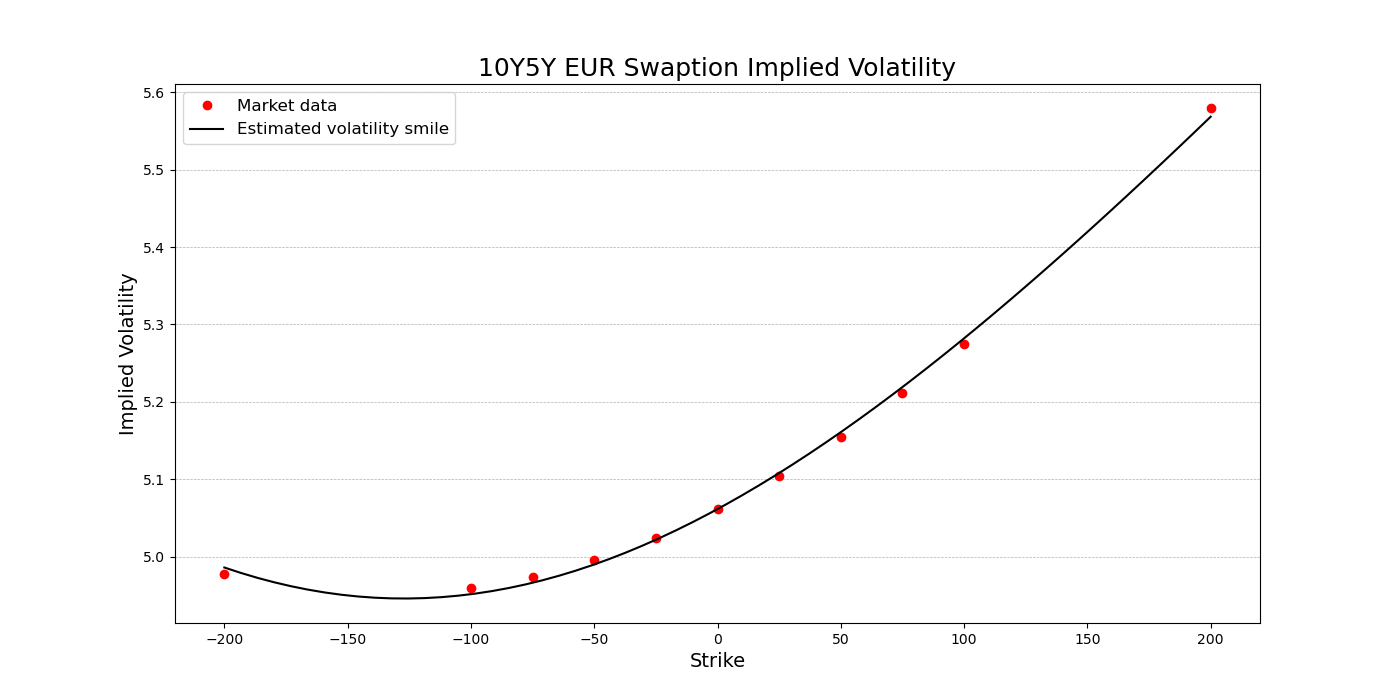
\includegraphics[scale =0.22]{/Users/nannaingemannohrt/Desktop/master_thesis/main/plots/10Y5Y_est.png}
        \caption{Volatility Surface EUR swaption 10Y5Y}
        \label{fig:10Y5Y_}
    \end{subfigure}
    \begin{subfigure}{0.43\textwidth}
        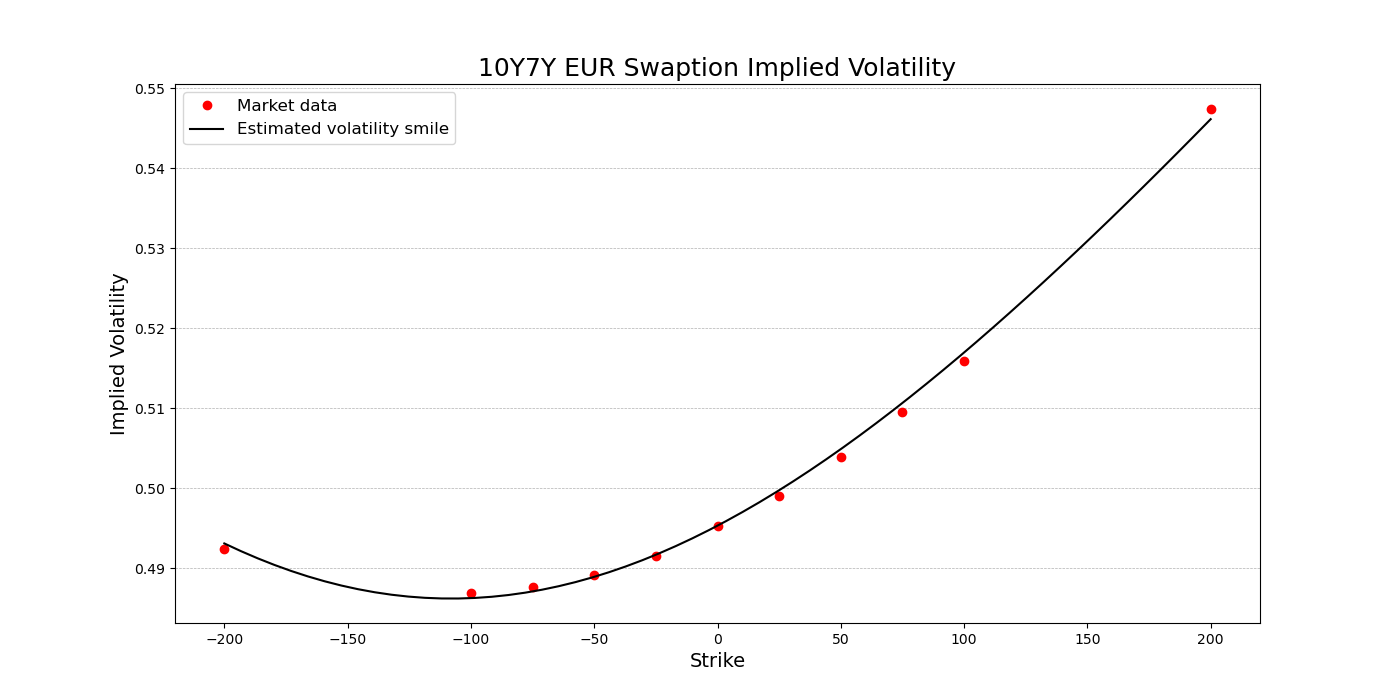
\includegraphics[scale =0.22]{/Users/nannaingemannohrt/Desktop/master_thesis/main/plots/10Y7Y_est.png}
        \caption{Volatility Surface EUR swaption 10Y7Y}
        \label{fig:10Y7Y_}
    \end{subfigure}\hfill
    \begin{subfigure}{0.43\textwidth}
        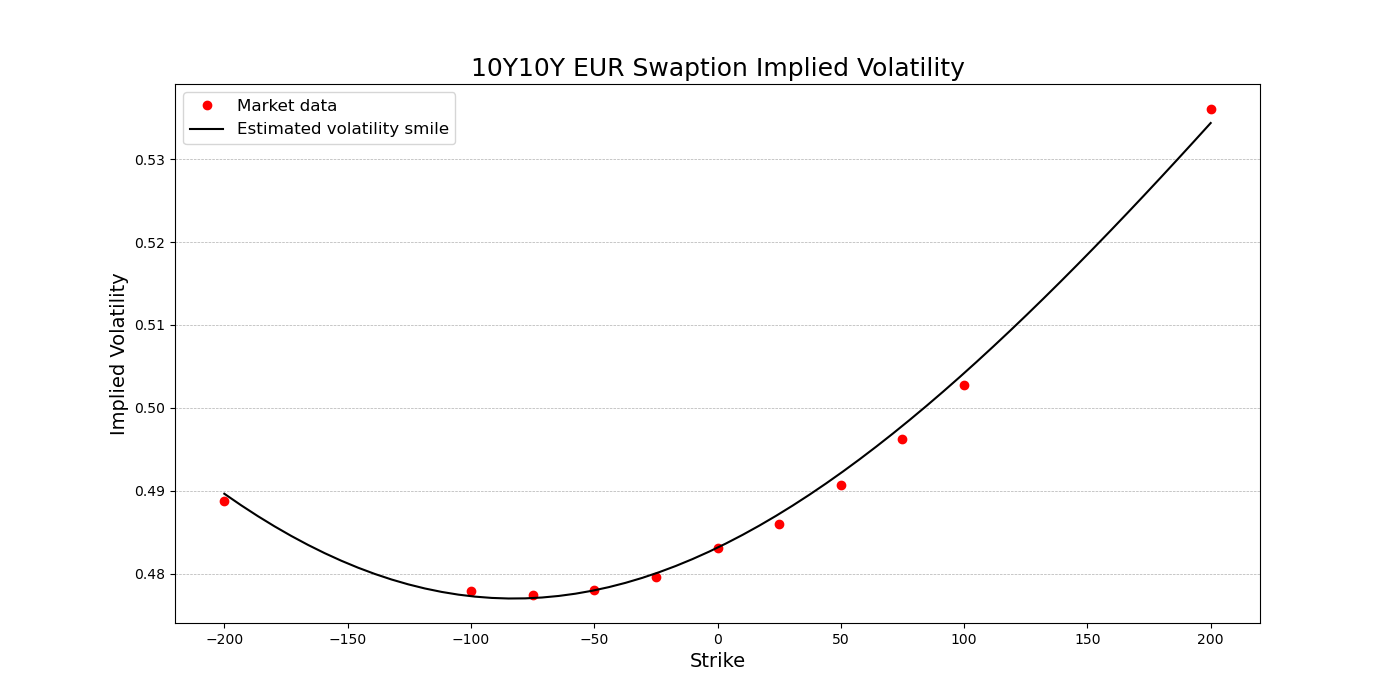
\includegraphics[scale =0.22]{/Users/nannaingemannohrt/Desktop/master_thesis/main/plots/10Y10Y_est.png}
        \caption{Volatility Surface EUR swaption 10Y10Y}
        \label{fig:10Y10Y_}
    \end{subfigure}

    \begin{subfigure}{0.43\textwidth}
        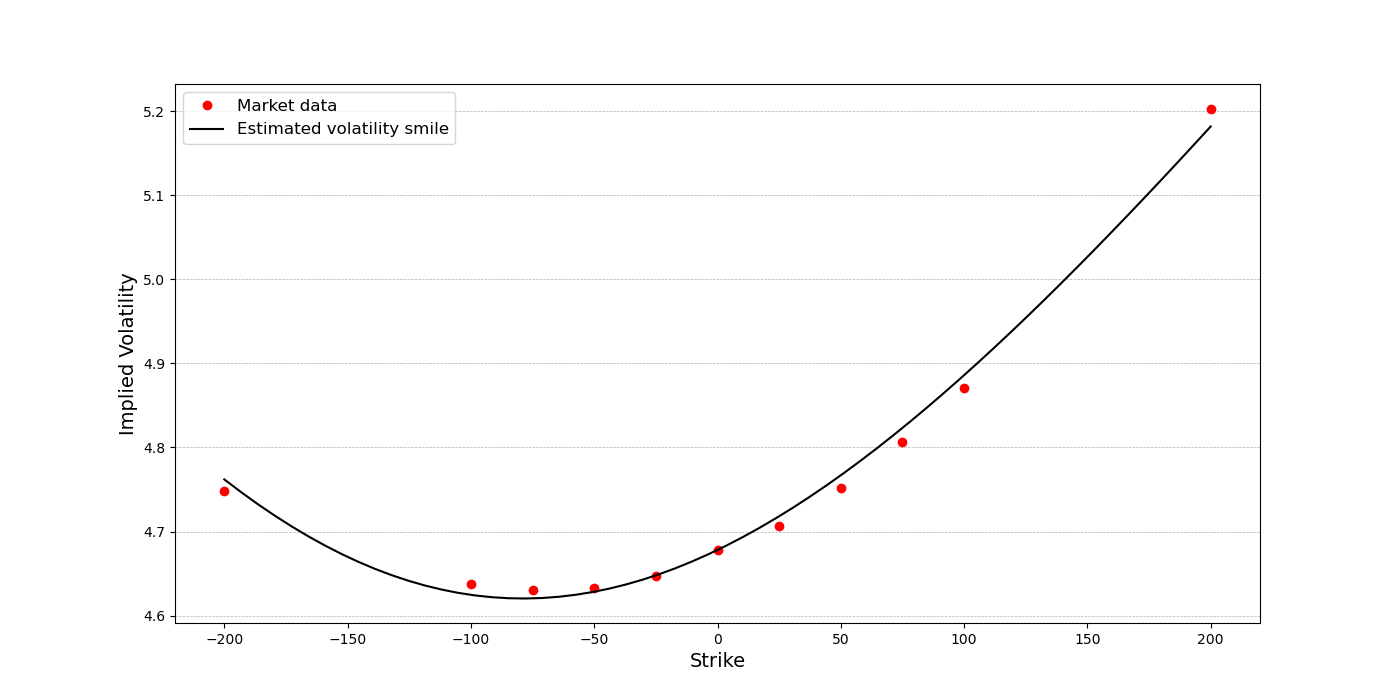
\includegraphics[scale =0.22]{/Users/nannaingemannohrt/Desktop/master_thesis/main/plots/10Y12Y_est.png}
        \caption{Volatility Surface EUR swaption 10Y12Y}
        \label{fig:10Y12Y_}
    \end{subfigure}\hfill
    \begin{subfigure}{0.43\textwidth}
        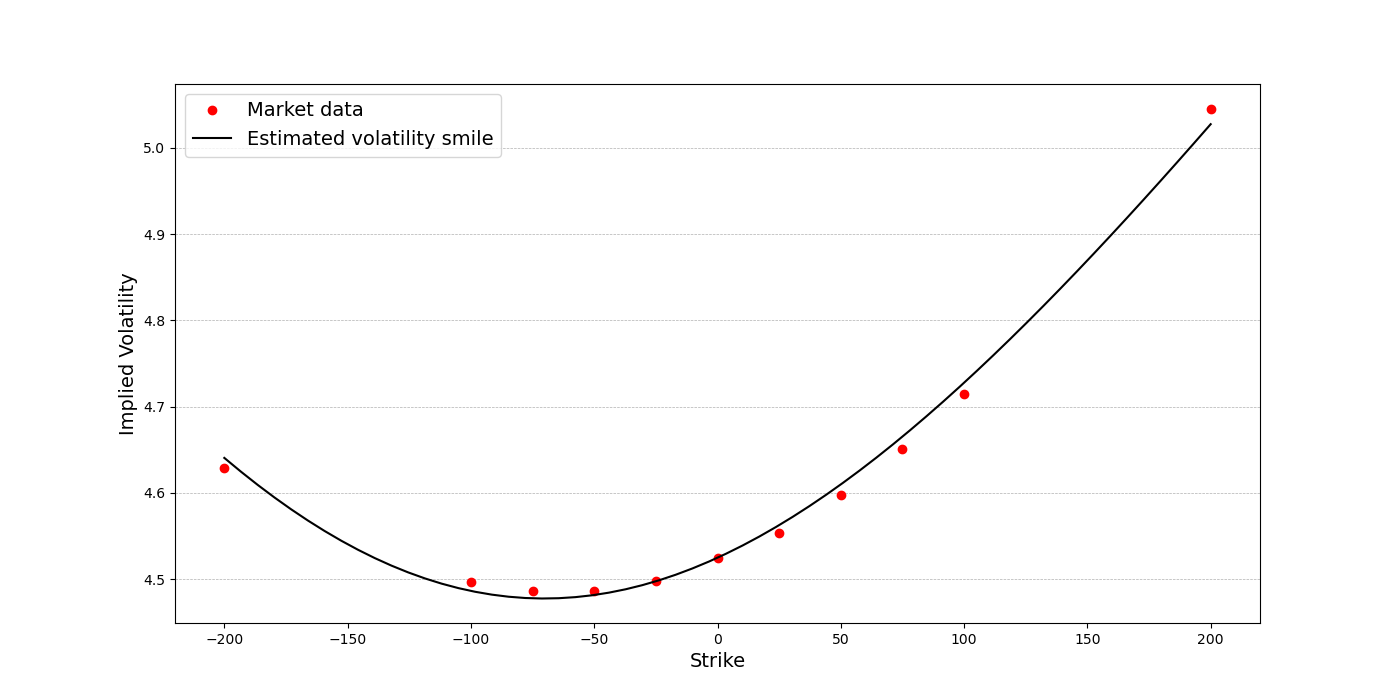
\includegraphics[scale =0.22]{/Users/nannaingemannohrt/Desktop/master_thesis/main/plots/10Y15Y_est.png}
        \caption{Volatility Surface EUR swaption 10Y15Y}
        \label{fig:10Y15Y_}
    \end{subfigure}
    \begin{subfigure}{0.43\textwidth}
        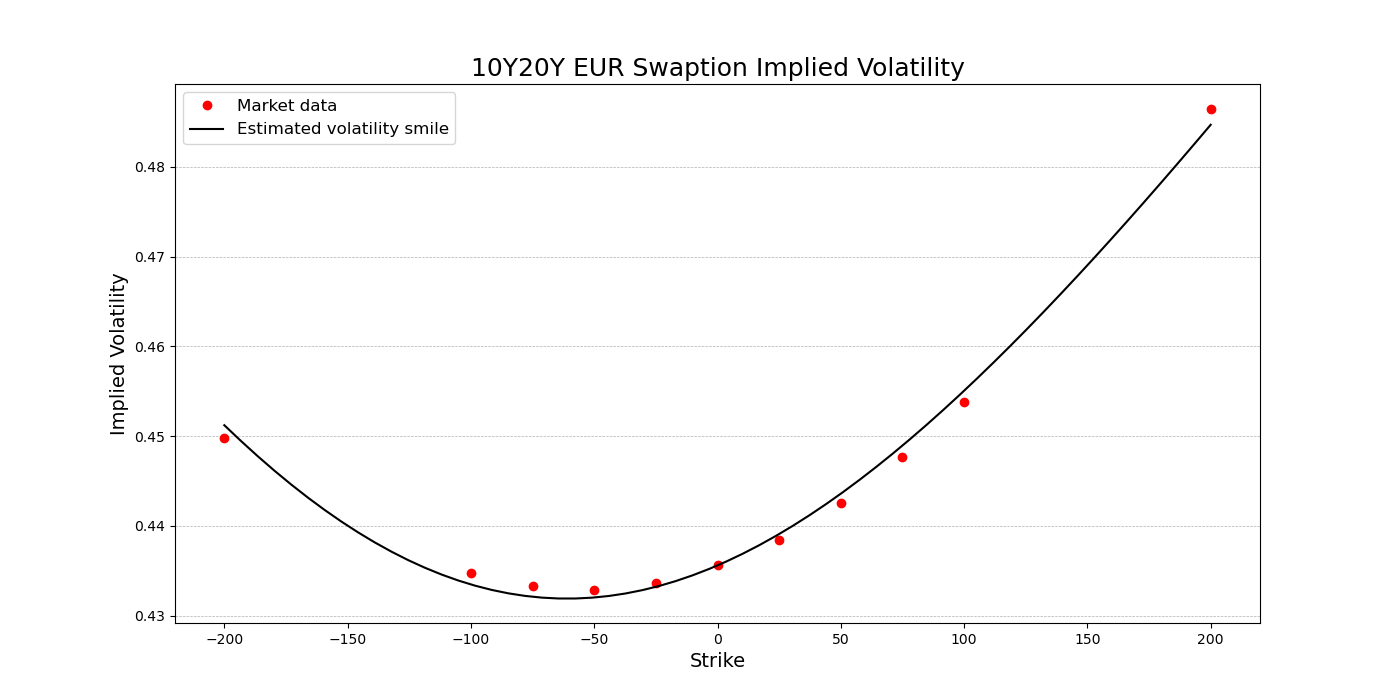
\includegraphics[scale =0.22]{/Users/nannaingemannohrt/Desktop/master_thesis/main/plots/10Y20Y_est.png}
        \caption{Volatility Surface EUR swaption 10Y20Y}
        \label{fig:10Y20Y_}
    \end{subfigure}\hfill
    \begin{subfigure}{0.43\textwidth}
        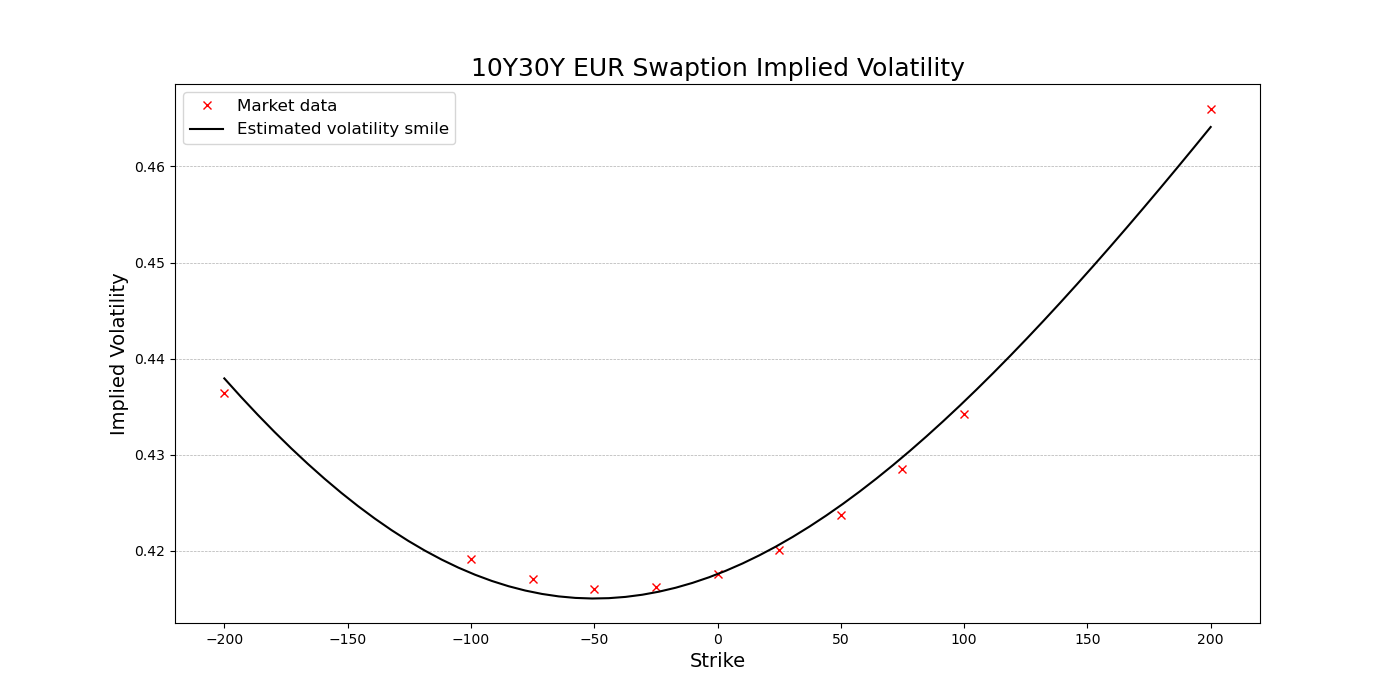
\includegraphics[scale =0.22]{/Users/nannaingemannohrt/Desktop/master_thesis/main/plots/10Y30Y_est.png}
        \caption{Volatility Surface EUR swaption 10Y30Y}
        \label{fig:10Y30Y_}
    \end{subfigure}

\end{figure}   